\chapter{The TRK Codebase: Core Algorithms}
\label{cha:code1}
% From Adam's thesis:
%For non-linear model curves, the tangent point must be found numerically. Depending on the functional form of yc(x; m), this point can be bracketed and found by any num-ber of numerical root-finding algorithms.4 We note that in the case of non-monotonic curves, there may be two or more such tangent points for each datapoint; in those cases, we choose the one that maximizes the joint probability.
% USE ALGORITHM ENVIRONMENTS
The previous chapter introduced all of the formalism needed to use the TRK statistic in principle, but how can TRK fits be done in practice? What are the implementational details? What options and configurations are available when using the TRK statistic? While the statistic itself was created by \textcite{trotter}, it was only implemented in the form of a genetic algorithm-based scientific codebase for testing. In order to have a production-quality codebase for the usage of TRK, I created a new suite of algorithms from scratch in C++, that completely overhauls how TRK fits are computed, including many additions and optimizations as compared to the previous codebase. With this new codebase, TRK can be used in a fully customizable, yet easy-to-use manner, with a host of options. The code and full documentation can be downloaded at \url{https://github.com/nickk124/TRK}.

The first part of this chapter will discuss the implementation of the central part of the TRK statistic, the TRK likelihood function $\mathcal{L}^\text{TRK}$ of Equation \eqref{eq:TRK}, that is maximized to obtain best fits. Here, I will explore my the algorithms that I use to determine the tangent points described by Equation \eqref{eq:tpoint}, and maximize $\mathcal{L}^\text{TRK}$ with respect to all model parameters---including slop---to obtain best fits. Following this, I will delve into the routine that is used to determine the optimum fitting scale $s_0$, using the formalism described in \S\ref{sec:TRKcorr}. From there, I will explore the Monte Carlo methods used to generate the full probability distributions and uncertainties of model parameters.

\section{Tangent Point Finding}
\label{sec:tgtfinder}
As shown in \S\ref{sec:tgtpts} and \S\ref{sec:likelihood}, for a given model curve $y_c(x;\vartheta_m)$ and datapoint $(x_n,y_n)$, the point where the convolved error ellipse of the datapoint described by the convolved error parameters $(\Sigma_{x,n}, \Sigma_{y,n})$ of Equation \eqref{eq:bigsigs} is tangent to the model curve, $(x_{t,n},y_{t,n})$, is a central part of the TRK likelihood $\mathcal{L}^\text{TRK}$ (Equation \eqref{eq:TRK}). Any time that the likelihood must be computed for a new set of model and slop parameters, all $N$ of these tangent points must be re-computed, and efficiently.

Recall that in order to determine such a tangent point $x_{t,n}$ (and therefore $y_{t,n}=y_c(x_{t,n};\vartheta_m)$), Equation \eqref{eq:tpoint} must be solved implicitly for $x_{t,n}$ in the general case of some nonlinear model. In more practical terms, this means that the root(s) along the $x-$axis of the left hand side of Equation \eqref{eq:tpoint} are such tangent point(s). To determine these tangent points, I use (a slightly modified version of) the Two-Point Newton-Raphson algorithm created by \textcite{tiruneh2013two} to find the roots of Equation \eqref{eq:tpoint}. This algorithm has a number of benefits over other root-finding methods such as bisection and the traditional Newton-Raphson method, especially when dealing with complicated nonlinear functions that otherwise give convergence and speed issues. My pseudocode implementation of it is shown in Algorithm \ref{algo:tpNR}.%, and my primary modification to the method of Tiruneh et. al is that during the course of the algorithm, if it's possible to use the bisection root-finding algorithm, it will switch to that.
\begin{algorithm}
\label{algo:tpNR}
\caption{Modified Two-Point Newton-Raphson algorithm for finding a single tangent point.}
\DontPrintSemicolon
    \SetKwInOut{Input}{Input}
    \SetKwInOut{Output}{Output}
    \SetKwProg{Fn}{Function}{}{}
    \Fn{TwoPointNR}{
    \Input{Model parameters $\vartheta_m$, datapoint $(x_n,y_n)$, its convolved errors $(\Sigma_{x,n}, \Sigma_{y,n})$, and initial tangent point guess of $x_{\text{guess}}$.}
    \Output{$x_{t,n}$}
    \Begin{
    Initialize guess of $x_{k-1}=x_{\text{guess}}$ and $x_k=x_{\text{guess}} + \Sigma_{x,n}/\sqrt{10})$\;
        \While{not converged}{
            \textit{Main Two-Pt NR loop:}\;
            $\displaystyle y_{k-1} = [y_c(x_{k-1};\vartheta_m) - y_n]\dv{y_c(x_{k-1};\vartheta_m)}{x}\Sigma_{x,n}^2 + (x_{k-1}-x_n)\Sigma_{y,n}^2$\;
            \vspace{0.3cm}$\displaystyle y_{k} = [y_c(x_{k};\vartheta_m) - y_n]\dv{y_c(x_{k};\vartheta_m)}{x}\Sigma_{x,n}^2 + (x_{k}-x_n)\Sigma_{y,n}^2$\;
            \vspace{0.3cm}$\displaystyle\dv{y_k}{x}=\left(\dv{y_c(x_{k};\vartheta_m)}{x}\right)^2 + [y_c(x_{k};\vartheta_m) - y_n]\dv[2]{y_c(x_{k};\vartheta_m)}{x}\Sigma_{x,n}^2+\Sigma_{y,n}^2$\;
            \vspace{0.3cm}$\displaystyle r=1 - \frac{y_k}{y_{k-1}}\left(\frac{y_k-y_{k-1}}{x_k-x_{k-1}}\bigg/\dv{y_k}{x}\right)$\;
            \vspace{0.3cm}$\displaystyle x_{k+1}=\left(1-\frac{1}{r}\right)x_{k-1}+\frac{x_k}{r}$\;
            % \textit{Stops Two-Pt NR and performs bisection root finding routine if possible:}\;
            % \If{$y_ky_{k-1}<0$}{
            %     $X = \{x_k,x_{k-1}\}$\;
            %     \Return{\textit{Bisection}(\textit{left bound}$=\min X$, \textit{right bound}$=\max X$)}\;
            % }
            $x_{k-1}=x_k,\,\,\, x_k=x_{k+1}$\;
        }
        \Return{$x_{t,n}=x_k$}
    }
    }
\end{algorithm}

It is essential to note that for certain non-monotonic, nonlinear models, there can easily be multiple tangent points for a given datapoint; see Figure \ref{fig:multtgt} as an example. In this case, I take the tangent point that maximizes the joint posterior probability\footnote{I.e. for some $n^\text{th}$ datapoint, the joint posterior probability is the $n^\text{th}$ term in the product of Equation \eqref{eq:TRK}.} as the tangent point to be used when evaluating the likelihood. However, only using the rootfinder of Algorithm \ref{algo:tpNR} once per datapoint is insufficient, as some initial guess for the algorithm will always only return the same, single tangent point. In order to reliably determine \textit{all} possible tangent points for a given datapoint, to properly maximize the likelihood, I use a logical routine described in Algorithm \ref{algo:tpFinder}. The goal of this routine is to determine various initial guesses to supply to the root-finder until all possible tangent point-finding options have been exhausted. To begin this algorithm, the root finder is used with the default initial guess to determine the first tangent point. From here, I use a quadratic approximation (of Equation \eqref{eq:tpoint}) through this first tangent point to approximate up to two more tangent points, and use these two approximate points as initial guesses for the root finder, which will determine the remaining roots\footnote{I also implemented a few modifications to this to account for certain edge cases (see Algorithm \ref{algo:tpFinder}).}. In general, I have found that non-periodic functions generally have no more than three tangent points for a given datapoint. Finally, I note that in the current C++ implementation of the TRK suite, the option to parallelize the determination of all $N$ tangent points for a given evaluation of $\mathcal{L}^\text{TRK}$ is provided\footnote{Parallelizing the tangent-point finder isn't always advisable for simple, linear models, as the two-point Newton-Raphson routine runs so fast with these models that the computational overhead for starting and stopping each tangent point's computational thread is greater than the power needed to actually find the tangent point itself. As such, this feature is most useful for nonlinear models.}.
\begin{figure}
    \centering
    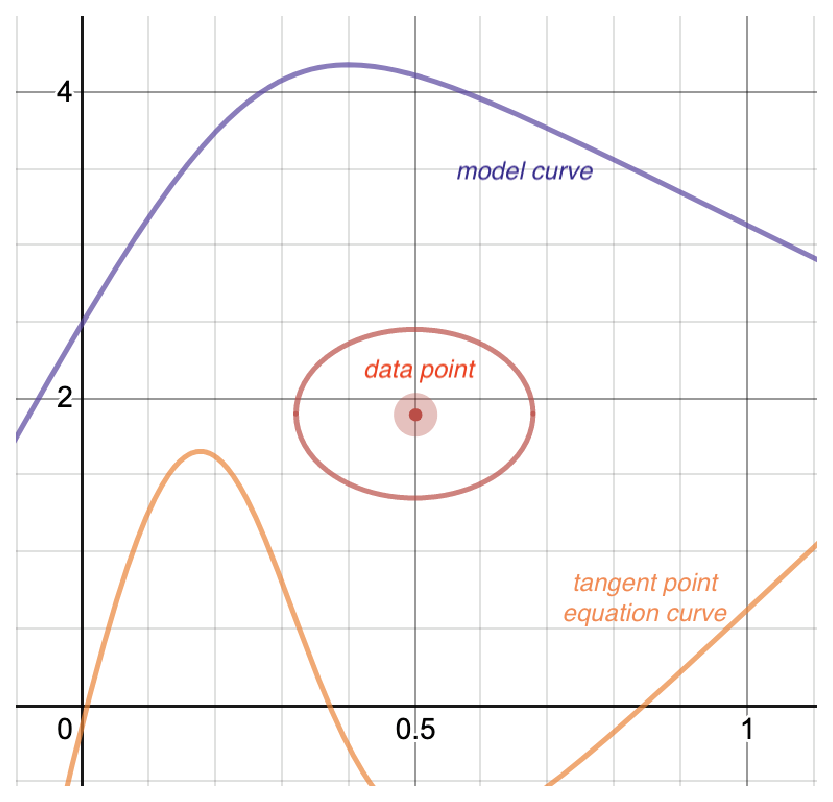
\includegraphics[width=0.6\linewidth]{figures/multtgtexample.eps}
    \caption{Example of a model curve $y_c(x;\vartheta_m)$ (purple, top) and datapoint $(x_n,y_n)$ with convolved error ellipse (red, middle) described by $(\Sigma_{x,n}, \Sigma_{y,n})$ where there are multiple points where $y_c$ is tangent to the ellipse. This translates to there being multiple solutions/roots to/of Equation \eqref{eq:tpoint}, which is plotted in orange at the bottom.}
    \label{fig:multtgt}
\end{figure}
\begin{algorithm}
\label{algo:tpFinder}
\caption{Find all possible tangent points for a given model and datapoint.}
\DontPrintSemicolon
    \SetKwInOut{Input}{Input}
    \SetKwInOut{Output}{Output}
    \SetKwProg{Fn}{Function}{}{}
    \Fn{FindAllTangentPoints}{
    \Input{Model parameters $\vartheta_m$, datapoint $(x_n,y_n)$, and its convolved errors $(\Sigma_{x,n}, \Sigma_{y,n})$.}
    \Output{Array of all tangent points $\{x_{t,n}^{i}\}$.}
    \Begin{
    Initialize empty $\{x_{t,n}^{i}\}$, and initialize $x_{\text{guess},0} = x_n$.\;
        \While{not all tangent points $x_{t,n}^{i}$ found}{
            \textit{First tangent point is the one that Two-Point Newton Raphson finds:}\;
            Append $x_{t,n}^\text{new} = $\textit{TwoPointNR}$(x_{\text{guess}} = x_{\text{guess},0})$ to $\{x_{t,n}^{i}\}$\;
            \If{New root found is same as one from previous iteration}{
                \textbf{break}\;
            }
            \If{TwoPointNR oscillating between two tangent points $x_1,x_2\in\{x_{t,n}^{i}\}$)}{
                $x_\text{mid} = $\textit{TwoPointNR}$[x_{\text{guess}} = $\textit{Midpoint}$(x_1,x_2)]$ to $\{x_{t,n}^{i}\}$\;
                {$\{x_{t,n}^{i}\} = \{x_1,x_2,x_\text{mid}\}$}\;
                \textbf{break}\;
            }
            
            \textit{Use quadratic approximation through $x_{t,n}^\text{new}$ to approximate two more tangent points if possible (see Algorithm \ref{algo:quadapprox}):}\;
            $\{x_{t,n}^\text{approx}\} = $\textit{QuadraticApprox}$(x_{t,n}^\text{new})$\;
            \If{$\{x_{t,n}^\text{approx}\}$ has 2 additional, approximate tangent points $x_\text{guess,1}, x_\text{guess,2}$}{
                Let $(x_\text{guess,1}, x_\text{guess,2}) = $these two new approximate tangent points\;
                \If{$x_{t,n}^\text{new}\in \{x_\text{guess,1}, x_\text{guess,2}\}$}{
                    $x_1 = $\textit{TwoPointNR}$(x_{\text{guess}} = x_\text{guess,1})$\;
                    $x_2 = $\textit{TwoPointNR}$(x_{\text{guess}} = x_\text{guess,2})$\;
                    {$\{x_{t,n}^{i}\} = \{x_1,x_2,x_{t,n}^\text{new}\}$}\;
                    \textbf{break}\;
                }
                \Else{
                    $x_{\text{guess},0} = $\textit{Median}$(x_{t,n}^\text{new},x_\text{guess,1}, x_\text{guess,2})$\;
                }
            }
            \If{$\{x_{t,n}^\text{approx}\}$ contains no new tangent points}{
                $x_\text{min} = \min\{x_n\}$, $x_\text{max} = \max\{x_n\}$
                $x_\text{left}= $\textit{TwoPointNR}$(x_{\text{guess}} = x_\text{min})$\;
                $x_\text{right}= $\textit{TwoPointNR}$(x_{\text{guess}} = x_\text{max})$\;
                Append $x_\text{left}, x_\text{right}$ to $\{x_{t,n}^{i}\}$\;
                \textbf{break}\;
            }
            \ElseIf{Two tangent points $x_1,x_2$ found in total, but $\{x_{t,n}^\text{approx}\}$ contains no new points}{
                {$\{x_{t,n}^{i}\} = \{x_1,x_2\}$}\;
                \textbf{break}\;
            }
        }
       % Remove duplicates within $\{x_{t,n}^{i}\}$\;
        \Return{$\{x_{t,n}^{i}\}$}\;
    }
    }
\end{algorithm}
\begin{algorithm}
\label{algo:quadapprox}
\caption{Use a quadratic approximation about a found tangent point to determine guesses for any additional unknown tangent points.}
\DontPrintSemicolon
    \SetKwInOut{Input}{Input}
    \SetKwInOut{Output}{Output}
    \SetKwProg{Fn}{Function}{}{}
    \Fn{QuadraticApprox}{
    \Input{Model parameters $\vartheta_m$, datapoint $(x_n,y_n)$, its convolved errors $(\Sigma_{x,n}, \Sigma_{y,n})$, and tangent point $x_{t,n}$ determined by Two-Point Newton Raphson root-finder.}
    \Output{Approximations of additional unknown tangent points $\{x_{t,n}^\text{approx}\}$, if any remain.}
    \Begin{
    Initialize empty array of possible approximate tangent points $\{x_{t,n}^\text{approx}\}$\;
    Approximate $\displaystyle y_c(x)\approx y_c(x_{t,n}) + \dv{y_c(x_{t,n})}{x} \left(x-x_{t,n}\right) +\frac{1}{2}\dv[2]{y_c(x_{t,n})}{x}\left(x-x_{t,n}\right)^2$\;
    Use this approximation for $y_c$ with Equation \eqref{eq:tpoint} to get a cubic equation for $\{x_{t,n}^\text{approx}\}$.\;
    \If {The discriminant of this cubic equation $ > 0$}{
        \textit{There exists two real and distinct additional approximate tangent points:}\;
        Use a cubic equation solver to analytically determine the two additional approximate tangent points, and append them to $\{x_{t,n}^\text{approx}\}$.\;
    }
    \Else {
    \textit{There exists no additional real approximate tangent points; the initial point $x_{t,n}$ found is the only one.}\;
    }
    \Return{$\{x_{t,n}^\text{approx}\}$}
    }
    }
\end{algorithm}

\section{Likelihood Maximization}
\label{sec:simplex}

The best fit at some scale $s$ is defined to be the model parameters $\vartheta_m$ and slop parameters $(\sigma_x,\sigma_y)$ that maximize the TRK likelihood $\mathcal{L}^\text{TRK}$ of Equation \eqref{eq:TRK}\footnote{The method used to determine the optimum fitting scale $s_0$ will be covered in \S\ref{sec:scaleop}.}; however, as described in \S\ref{sec:tgtpts}, in practice the TRK suite \textit{minimizes} $\chi^2_\text{TRK}\equiv-2\ln \mathcal{L}^\text{TRK}$ to determine best fits. For less general statistics where slop is not included in the likelihood, $-2\ln\mathcal{L}$ is often minimized using methods such as the Gauss-Newton algorithm, e.g. \textcite{maples2018robust}. The Gauss-Newton algorithm is usually quick to converge because it uses the partial derivatives of the model function with respect to the model parameters. However, because an explicit expression is required for each derivative, this method does \textit{not} translate over to the TRK statistic, as the dependence of the model curve $y_c$ on the slop parameters $(\sigma_x, \sigma_y)$ cannot be explicitly written down in the general case. Because $\chi^2_\text{TRK}$ must be minimized not only with respect to the model parameters, but also the slop parameters, Gauss-Newton, or any other method that requires explicit parameter derivatives, is not an option. 

Instead, the TRK suite uses a modified version of the Downhill Simplex algorithm of \textcite{NelderMead65} to minimize $\chi^2_\text{TRK}$, with explicit implementation given in Algorithm \ref{algo:simplex}. The basic mechanism of this algorithm is that given $\mathcal{M}$ model and slop parameters, a \textit{simplex}\footnote{A simplex is essentially a higher-dimensional generalization of a triangle.} with $\mathcal{M}+1$ vertices is initialized and evolves within parameter space along the surface of $\chi^2_\text{TRK}$, with its evolution depending on the values of $\chi^2_\text{TRK}$ at its various vertices, in order to find the minimum of $\chi^2_\text{TRK}$. This method is advantageous due to it's general reliability, and the fact that no matter the number of parameters in the model, the only function that the user need supply to the algorithm is the model curve\footnote{However, the user still needs to supply the first two $x-$derivatives of $y_c$, for the tangent point-finding routine of \S\ref{sec:tgtfinder}.}, as opposed to an $\mathcal{M}$-parameter model requiring the user to supply $\mathcal{M}$ partial derivatives of the model, as in the Gauss-Newton algorithm\footnote{We note that for complicated nonlinear and/or high dimensional models, the simplex method can be fairly dependent on the user-supplied initial guess for the model and slop parameters, given that such models are often fraught with local minima.}. 
\begin{algorithm}
\label{algo:simplex}
\caption{Modified Nelder-Mead Downhill Simplex algorithm for determining best fits according to $\chi^2_\text{TRK}\equiv\mathcal{L}^\text{TRK}$. Note that if a simplex vertex $v$ enters a region of parameter space forbidden by any provided bounded parameter priors, $\chi^2_\text{TRK}(v)\sim+\infty$.}
\DontPrintSemicolon
    \SetKwInOut{Input}{Input}
    \SetKwInOut{Output}{Output}
    \SetKwProg{Fn}{Function}{}{}
    \Fn{DownhillSimplex}{
        \Input{Model $y_c$, initial guess for model and slop parameters $\{\vartheta_m,(\sigma_x,\sigma_y)\}^\text{guess}$ of dimension $\mathcal{M}$, dataset $\{x_n,y_n\}$ with error bars $\{\sigma_{x,n}, \sigma_{y,n}\}$, given some fit scale $s$}
        \Output{Best fit parameters $\{\vartheta_m,(\sigma_x,\sigma_y)\}$}
        \Begin{
            Initialize simplex $\Delta$ with $\mathcal{M}+1$ vertices $v_i, i\in\{0,\cdots,\mathcal{M}\}$ about $v_0=\{\vartheta_m,(\sigma_x,\sigma_y)\}^\text{guess}$, with values of $\ctrkk(v_i)\equiv\chi^2_i$ at each $v_i$\;
            \While{\textit{StdDev}$\{\chi^2_i\} > $ tolerance}{
                \textit{Each iteration of this is one simplex step.}\;
                Reorder the the vertices $v_i$ of $\Delta$ with respect to ascending ordering of $\ctrkk(v_i)\equiv\chi^2_i$.\;
                Compute centroid excluding ``worst'' vertex $v_\mathcal{M}$, $\displaystyle c \equiv\frac{1}{\mathcal{M}}\sum\limits_{i=0}^{\mathcal{M}-1}v_i$.\;
                \textit{Reflect}: Compute reflection point of $v_\mathcal{M}$, $v_r\equiv c + \alpha(c-v_\mathcal{M})$\;
                    \If{$\chi^2_0 \leq \chi^2_r < \chi^2_{\mathcal{M}-1}$}{
                        $v_\mathcal{M}\rightarrow v_r$\;
                        \textbf{continue}\;
                }
                \If{$\chi^2_r < \chi^2_0$}{
                    \textit{Expand}$(\Delta)$ (see Algorithm \ref{algo:simplexsteps} in \S\ref{app:algos})\;
                    \textbf{continue}\;
                }
                \If{$\chi^2_r \geq \chi^2_{\mathcal{M}-1}$}{
                    \textit{Contract}$(\Delta)$ (see Algorithm \ref{algo:simplexsteps} in \S\ref{app:algos})\;
                    \textbf{continue}\;
                }
                \textit{Shrink}$(\Delta)$ (see Algorithm \ref{algo:simplexsteps} in \S\ref{app:algos})\;
            }
            \textit{pegSlopToZero}$(\Delta)$\;
            \textit{makeSlopPositive}$(\Delta)$  \textit{(see bullet point \ref{enum:newsimplex2} on pg. \pageref{enum:newsimplex1})}\;
            \Return{Best fit $\{\vartheta_m,(\sigma_x,\sigma_y)\}\equiv v_\mathcal{M}$}\;
        }
    }
\end{algorithm}
For my implementation of the Nelder-Mead algorithm, I also made the following modifications:
\begin{enumerate}
    \item \label{enum:newsimplex1}Any user-supplied prior probability distributions that place hard upper and/or lower bounds on model parameters will act as ``walls'' for the evolution of the simplex, i.e. if the simplex enters a region of a forbidden value of a model parameter, $\chi^2_\text{TRK}$ will evaluate as numerical infinity.
    \item \label{enum:newsimplex2}Once the best fit model and slop parameters have been determined by the minimization of $\chi^2_\text{TRK}$, small values of slop are ``pegged'' to zero if they are within a given tolerance, for the usage of the scale optimization algorithm described in \S\ref{sec:scaleop}. Additionally, any negative best fit slop values $(\sigma_x,\sigma_y)$ are made positive for the final best fit, because although the simplex explores parameter space with respect to $(\sigma_x,\sigma_y)$, these terms are always squared when they appear in the likelihood (Equation \eqref{eq:TRK}), so a fitted negative value is equivalent to a positive.
\end{enumerate}

\section{Scale Optimization}
\label{sec:scaleop}

As described in \S\ref{sec:scalability}, the TRK statistic/likelihood is \textit{not} scalable by default, i.e. multiplying a dataset along the $y$-axis by some numerical factor $s$ will result in different best fits for various values of $s$. As such, we are presented with the problem of determining the \textit{global} optimum scale $s=s_0$ to perform fits for a given dataset and model. Such a method was explored schematically in \S\ref{sec:TRKcorr} on pg. \pageref{par:scaleopscheme} as presented by \textcite{trotter}, and in the following section I will present the explicit implementational details of the \textit{scale optimization algorithm}. 

Given some dataset and model, from Equation \eqref{eq:r2TRK}, we must begin by determining the \textit{minimum} and \textit{maximum} fitting scales $a$ and $b$ as described in \S\ref{sec:TRKcorr}. Recall from this section that $a$ is the scale where as $s\rightarrow a^+$, the slop in the $x$-direction, $\sigma_x\rightarrow 0$. Similarly, $b$ is the scale where as $s\rightarrow b^-$ the $y-$slop $\sigma_y\rightarrow 0$. An example of this behavior is presented in Figure \ref{fig:slopvscale}, where I plot best fit slop values $\sigma_x$, $\sigma_y$ for various values of $s$, given a linear model\footnote{Specifically, for the $c_1$ vs. $c_2$ spectral dust extinction model and dataset described in \S\ref{sec:extincfits}.}.
\begin{figure}
    \centering
    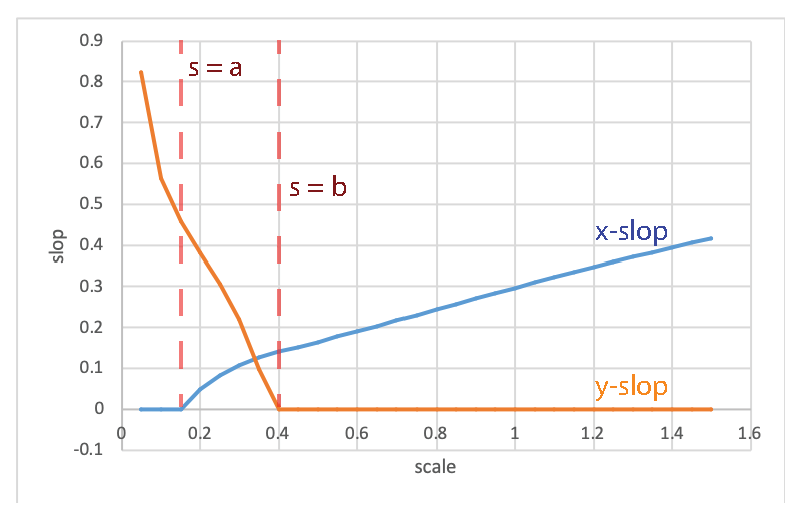
\includegraphics[width=0.8\linewidth]{figures/slopvscale.eps}
    \caption{Example of slop/extrinsic scatter $(\sigma_x,\sigma_y)$ dependence on fitting scale $s$ (for some linear model). Note that as is predicted in \S\ref{sec:TRKcorr}, there exist minimum and maximum scales $s=a$ and $s=b$ (respectively) such that $\lim\limits_{s\rightarrow a^+}\sigma_x = 0$ and $\lim\limits_{s\rightarrow b^-}\sigma_y = 0$.}
    \label{fig:slopvscale}
\end{figure}

In order to determine the scale extrema $a$ and $b$ for a given model and dataset, I implemented a type of bracketing/bisection method that, by running fits at various scales (using the Downhill Simplex routine of Algorithm \ref{algo:simplex}) and observing best fit slop values, finds the exact scales where the two slops go to zero. This method determines $a$ first, and then $b$; I present the method for determing $a$ as Algorithm \ref{algo:minscale}, and the similar method for determining $b$ is given as Algorithm \ref{algo:maxscale} in \S\ref{app:algos}. Note that I also make several modifications for improved efficiency, such as using best fit values for $\sigma_y$ obtained from determining $a$ to start the routine for determining $b$ at a better initial guess. I also provide the option to find the two scale extrema at the same time using parallel computing (in the current, C++ implementation of the TRK suite).
\begin{algorithm}
\label{algo:minscale}
\caption{Bracketing/Bisection-type method for determining minimum fitting scale $a$ for some model and dataset.}
\DontPrintSemicolon
    \SetKwInOut{Input}{Input}
    \SetKwInOut{Output}{Output}
    \SetKwProg{Fn}{Function}{}{}
    \Fn{FindMinimumScale}{
        \Input{Model $y_c$ and dataset $\{x_n,y_n\}$ with error bars $\{\sigma_{x,n}, \sigma_{y,n}\}$.}
        \Output{Minimum fitting scale $a$.}
        \Begin{
            \textit{Determine brackets $(l,r)$ for min scale $a$:}\;
            Initialize bisection brackets $l = s = 0, r = s = 1$ and $s_\text{trial} = s = 1$.\;
            $\sigma_x(s_\text{trial}) \leftarrow $\textit{ DownhillSimplex}($s=s_\text{trial}$)\;
            Initialize step modifier $\alpha = 0.5\times s_\text{trial}$.\;
            \If{$\sigma_x(s_\text{trial}) > 0$}{
                $r = s_\text{trial}$\;
                $l_\text{trial}=s_\text{trial}$\;
                $\sigma_x(l_\text{trial})=$\textit{DownhillSimplex}($s=l_\text{trial}$)\;
                \While{$\sigma_x(l_\text{trial}) > 0$}{
                    $l_\text{trial} = l_\text{trial}-\alpha$\;
                    $\sigma_x(l_\text{trial})=$\textit{DownhillSimplex}($s=l_\text{trial}$)\;
                    $\alpha = 0.5\times\alpha$\;
                    $r=l_\text{trial}$\;
                }
                $l=l_\text{trial}$\;
            }
            \ElseIf{$\sigma_x(s_\text{trial}) = 0$}{
                $l = s_\text{trial}$\;
                $r_\text{trial}=s_\text{trial}$\;
                $\sigma_x(l_\text{trial})=$\textit{DownhillSimplex}($s=l_\text{trial}$)\;
                \While{$\sigma_x(r_\text{trial}) = 0$}{
                    $r_\text{trial} = r_\text{trial}+\alpha$\;
                    $\sigma_x(r_\text{trial})=$\textit{DownhillSimplex}($s=r_\text{trial}$)\;
                    $l=r_\text{trial}$\;
                }
                $r=r_\text{trial}$\;
            }
            \textit{Use bisection to determine $a$ now that we have brackets $(l,r)$:}\;
            $a_\text{trial} = (l+r)/2$\;
            $\sigma_x(a_\text{trial})=$\textit{DownhillSimplex}($s=a_\text{trial}$)\;
            \While{$\abs{l-r}\geq$ tolerance1 AND $\sigma_x(a_\text{trial})\geq$ tolerance2}{
                $a_\text{trial} = (l+r)/2$\;
                $\sigma_x(a_\text{trial})=$\textit{DownhillSimplex}($s=a_\text{trial}$)\;
                \If{$\sigma_x(a_\text{trial})>0$}{
                    $r = a_\text{trial}$\;
                }
                \ElseIf{$\sigma_x(a_\text{trial})=0$}{
                    $l = a_\text{trial}$\;
                }
            }
            \Return{$a=a_\text{trial}$}
        }
    }
\end{algorithm}

Now that the method for determining the scale extrema $a$ and $b$ for a certain model and dataset has been presented, the optimum scale $s_0$ needs to be determined. From \S\ref{sec:TRKcorr}, in order to determine successive approximations for $s_0$ until convergence, Equation \eqref{eq:r2TRKnewscalenonlin} must be repeatedly solved for $s_0^{(2)}$ given the previous iteration's solution $s_0^{(1)}$. I begin this process with $s_0^{(1)}=(a+b)/2$, and then successively solve Equation \eqref{eq:r2TRKnewscalenonlin} numerically while setting $s_0^{(1)} = s_0^{(2)}$ after each iteration.

In practice, Equation \eqref{eq:r2TRKnewscalenonlin} is solved by rewriting it as
\begin{align}\label{eq:r2TRKnewscalenum}
\tilde{R}^2_{\mathrm{TRK}}(s_0^{(2)};s_0^{(1)}, a, b) & \equiv \frac{1}{N}\sum_{n=1}^{N}\tan^2\left(\frac{\pi}{4}-\frac{\left|\arctan  (s_0^{(1)}\tan\theta_{t,n;a})-\arctan  (s_0^{(1)}\tan\theta_{s_0^{(2)}})\right|}{2}\right) \nonumber \\
& -
\frac{1}{N}\sum_{n=1}^{N}\tan^2\left(\frac{\pi}{4}-\frac{\left|\arctan  (s_0^{(1)}\tan\theta_{s_0^{(2)}})-\arctan  (s_0^{(1)}\tan\theta_{t,n;b})\right|}{2}\right)\nonumber\\
& =0 \, ,
\end{align}
and numerically solving the equation for $s_0^{(2)}$ given the previous $s_0^{(1)} = s_0^{(2)}$ using a bisection root-finding routine, repeating as necessary until convergence\footnote{Here I use bisection instead of other root-finding algorithms (e.g. Newton-Raphson) because most of these other algorithms require derivatives of the function with respect to the independent variable. As the derivative of Equation \eqref{eq:r2TRKnewscalenum} with respect to $s_0^{(2)}$, for example, is ill-defined, the usage of bisection is a necessity. Furthermore, because this dependence of slop on scale has shown to be monatonic in all models that I have explored, bisection is perfectly suited for the task.}. I then set the final optimum scale $s_0$ to be the last iteration of $s_0^{(2)}$. This algorithm is presented in it's entirety as Algorithm \ref{algo:opscaler2} in \S\ref{app:algos}, on pg. \pageref{algo:opscaler2}.

\section{Model Parameter Distribution and Uncertainty Computation}
\subsection{Using Adaptive MCMC to Sample Parameter Distributions}
\label{sec:MCMC}
As a review, so far I have covered everything that is needed to determine best fit model and slop parameters for any given nonlinear model and dataset with intrinsic and extrinsic two-dimensional uncertainties. In practice, I run the scale optimization routine (Algorithms \ref{algo:minscale}, \ref{algo:maxscale}, and \ref{algo:opscaler2} sequentially) to determine the optimum fitting scale $s_0$, and then find the best fit model and slop parameters $\{\vartheta_m,(\sigma_x,\sigma_y)\}$ using the Nelder-Mead downhill simplex to maximize the TRK likelihood function $\mathcal{L}^\text{TRK}$ (Algorithm \ref{algo:simplex}). In reality, the \textit{uncertainties} of the best fit model parameters (and possibly the slop parameters) are also often desired as a result of a fit, if not their complete \textit{posterior} probability distributions \footnote{The latter often when the distribution(s) of the parameter are not simply Gaussian.}. Furthermore, if any prior information is known about the model parameters in the form of \textit{prior} probability distribution(s), it can be essential to introduce them to the computation of the posteriors, following Bayes' Theorem (Equation \eqref{eq:bayes}).

There are a number of methods that can be used to sample a parameter's (posterior probability) distribution, but the types of methods that offer some of the most flexibility, speed, and support for priors are  Markov Chain Monte Carlo, or \textit{MCMC} methods. MCMC methods are a class of algorithms used to sample probability distributions, and they fall under the broad umbrella of \textit{Monte Carlo Methods} which are, generally speaking, the usage of the ability of computers to rapidly generate random numbers to simulate useful numerical results, that are often otherwise computationally intractable with more straight-forward methods. A simple example of a Monte Carlo method is the continuous sampling of a \textit{proposal} Gaussian distribution; as the number of samples becomes larger, the \textit{generated distribution} will converge to the proposal distribution. A \textit{Markov Chain} can generally be described as a process that continually changes from state to state following certain transition probability rules that are dependent on the previous state. Together, the moniker \textit{Markov Chain Monte Carlo} describes how a Markovian random walk is taken through parameter space to sample and generate the distribution of the parameters over time, according to chosen rules for the evolution and sampling. In turn, this sampling of the distribution can be used to estimate uncertainty, central tendency (e.g. mean, mode etc.), and other useful quantities. For the TRK algorithm suite, the specific MCMC method that we use is the adaptive version of the classic Metropolis-Hastings sampling algorithm of \textcite{hastings1970monte}, which will be described as follows\footnote{I chose Metropolis-Hastings sampling over other methods, e.g. Hamiltonian Monte Carlo, due to it's speed and because I have seen most model parameter distributions to be well behaved enough for Metropolis-Hastings to be sufficient for the purposes of this algorithm.}.

To begin, recall from \S\ref{sec:bayes} that the \textit{posterior probability distribution} of a model is the probability distribution of obtaining some values $\Theta\equiv\{\vartheta_m,(\sigma_x,\sigma_y)\}$ for the model (and slop) parameters given a dataset $D\equiv\{x_n,y_n,\sigma_{x,n},\sigma_{y,n}\}$. As such, in order to quantify any uncertainty of the predictions laid out by the best fit model parameters, the posteriors need to be examined. From Bayes' Theorem (Equation \eqref{eq:bayes}), then, sampling the posterior is \textit{equivalent} to (besides a factor of proportionality\footnote{Again, this constant factor is of no consequence because in most cases, we often don't care about the absolute probability of a some range of values for parameters, but rather the relative probability as compared to another range of possible values. Even if we did, we could integrate over the posterior to compute the constant of proportionality, as it is just a normalization constant found by the condition that $\int p(\Theta|D)\diff \Theta=1$.}) sampling the likelihood function multiplied by any priors\footnote{Note that if no priors are given for some or all of the parameters, the prior distribution(s) are \textit{uninformative}, or flat, i.e. $p(\Theta)=1$, such that the posterior is then directly proportional to the likelihood.}, i.e.
\begin{equation}
     P(\Theta|D)\propto\mathcal{L}^\text{TRK}(D|\Theta)p(\Theta)\,.
\end{equation}
Generally, the Metropolis-Hastings method works by iteratively generating a sequence of samples of parameters, that as the number of samples $R\rightarrow+\infty$, converges to the true probability distribution of the parameters. Given some sample $\Theta_i$, the possible distribution of the next potential sample $\Theta_t$, or the \textit{proposal distribution} $Q(\Theta_t|\Theta_i)$, is dependent on the value of $\Theta_i$ (which is why the sequence of samples is a Markov Chain). I note that by default, $Q$ is implemented as a Gaussian distribution, which could easily be changed if needed. The acceptance of this next potential sample is dependent on the proposal distribution: if it is accepted, it becomes the next step in the Markov Chain; if not, the sample is discarded and another potential sample is generated. The probability of acceptance for a potential parameter sample $\Theta_t$ is based off of the ratio between the posterior evaluated at the potential sample, and that at the previous sample $\Theta_i$; specifically, $\Theta_t$ is accepted if $\alpha \geq u$, where $\displaystyle\alpha\equiv \frac{\mathcal{L}^\text{TRK}(\Theta_t)p(\Theta_t)}{\mathcal{L}^\text{TRK}(\Theta_i)p(\Theta_i)}$ and $u\sim\mathcal{U}(0,1)$ ($\mathcal{U}$ indicates the uniform distribution)\footnote{\label{footnote:logpost}I note that in regions of parameter space that evaluate to extremely high likelihood, this ratio of posteriors $\displaystyle\frac{P(\Theta_t)}{P(\Theta_i)} = \frac{\mathcal{L}^\text{TRK}(\Theta_t)p(\Theta_t)}{\mathcal{L}^\text{TRK}(\Theta_i)p(\Theta_i)}$ can evaluate with computational underflow or overflow errors. As such, in practice the TRK suite samples in log space, i.e. some trial $\Theta_t$ is accepted given a previous $\Theta_i$ if $\ln\alpha=\ln\mathcal{L}^\text{TRK}(\Theta_t) - \ln\mathcal{L}^\text{TRK}(\Theta_i) + \ln p(\Theta_t) - \ln p(\Theta_i)\geq \ln u$, where again $u\sim\mathcal{U}(0,1)$; this helps combat such numerical errors \textcite{stackoverflowlogpostsoln}. (Observing Equation \eqref{eq:TRK}, these errors can occur due to having a large dataset, small error bars and/or slop, high or low datapoint weights---see footnote \ref{footnote:weighting} on page \pageref{footnote:weighting}---and/or other reasons.}.

The proposal distribution $Q(\Theta_t|\Theta_i)$ is proportional to the target \textit{true} posterior distribution $P(\Theta)$ (in our case we assume a Gaussian distribution for this, which can easily be changed), while the \textit{location} (i.e. mean) of $Q(\Theta_t|\Theta_i)$ is what changes from sample to sample (specifically, $Q(\Theta_t|\Theta_i)$ is centered on the most recent sample on the chain $\Theta_i$). The \textit{size}, or in other words the \textit{covariance matrix} $\Sigma$ and therefore standard deviations of $Q(\Theta_t|\Theta_i)$---the latter of which can be considered to be analogous to the step size(s) of the Markov Chain for each parameter, as will be shown shortly---on the other hand must be chosen prior to sampling, and will very much affect the quality and efficiency of the overall sampling. 

To see this behavior, consider some parameter $m$ that is Gaussian-distributed, that we wish to sample with the Metropolis-Hasting method. We need to choose the standard deviation/width $\sigma_m$ of the MCMC proposal distribution $Q(m)$ for the sampler, which we will refer to as the ``step size'' of the Markov Chain. We will use a fairly large sample count of $R=100,000$\footnote{Minus the ``burn-in'' of $10,000$ initial samples that are discarded, to allow for the Markov Chain to enter the majority of the distribution and not over-sample the outside.}, and run the sampler given three noticeably different values of $\sigma_m$. The results of these three separate samplings are shown in Figure \ref{fig:mcmcstepsize}; clearly, choosing the right values for the step sizes/proposal covariance matrix of an MCMC sampler is essential; ``step size'' values that are too large or too small can lead to terrible samplings\footnote{The technical reasons for the erroneous nature of such samplings are beyond the scope of this work, but it is related to the  ratio of the number of potential samples accepted by the Metropolis-Hastings criterion to the number of total samples attempted. Too high a step size leads to too many samples being accepted, while too low a step size leads to too few. Initially, I attempted to optimize the $M+2$ step sizes of the model and slop parameters with respect to this acceptance ratio, but this proved faulty for a number of reasons.}.
\begin{figure}
    \centering
    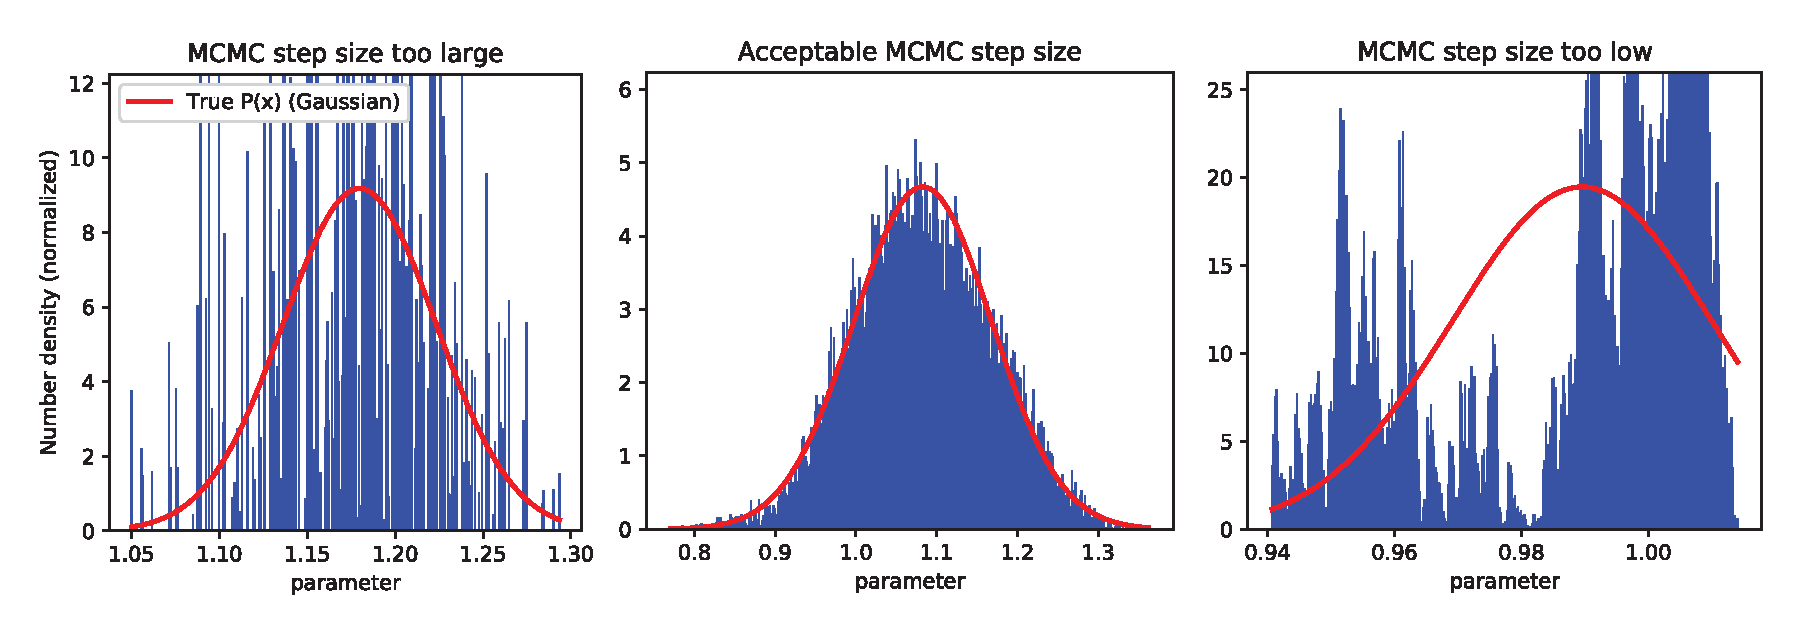
\includegraphics[width=1.0\linewidth]{figures/mcmcstepsizeall.eps}
    \caption{Histograms of MCMC Metropolis-Hastings samplings for a normal-distributed parameter $m$, with true Gaussian posterior plotted in red, given (Gaussian) proposal distribution widths/``step sizes'' of $\sigma_m=10$, $\sigma_m=0.1$, and $\sigma_m=0.0001$, from left to right, given a sample size of $R=100,000$. Note that even with such a high sample size, the choice of the step size for the model parameter's Markov Chain will \textit{drastically} change the quality of the sampling.}
    \label{fig:mcmcstepsize}
\end{figure}
However, it is very difficult to judge the quality of a choice of proposal distribution step sizes without running the full sampling itself. Because the TRK likelihood $\mathcal{L}^\text{TRK}$ requires running the tangent point-finding logic for all $N$ data-points at every evaluation of $\mathcal{L}^\text{TRK}$, and I have found that it usually takes $R\sim 100,000$ to get a decent sampling of the posterior, $2\times N\times 100,000$ calls to the tangent-point finding routine are required in order to sample the posterior distribution of the model and slop parameters of a given model and dataset\footnote{The factor of 2 here is due to the Metropolis-Hastings acceptance ratio requiring two calls to the posterior/likelihood function}. Even with parallelization and other optimizations, this requires a fair amount of computational work, especially if there are many datapoints and/or a complicated multi-dimensional model. As such, simply using trial-and-error to determine the best proposal distribution covariance matrix by iteratively running full samplings is computationally impractical, \textit{especially} if there are many model parameters, and therefore many step sizes that need tuning.

Because of this problem, I wished to efficiently automate the choosing of the proposal distribution covariance matrix, both to need as little user intervention and to require the lowest overall computation time as possible. To do so, I used the Adaptive MCMC algorithm of \textcite{haario2001adaptive}, which updates the (mean and covariance matrix of the) proposal distribution $Q$ while the sampling process is underway, according to the quality of the accumulating total sample. My implementation of the complete Adaptive MCMC sampler is shown as Algorithm \ref{algo:mcmc}.
\begin{algorithm}
\label{algo:mcmc}
\caption{Adaptive Metropolis-Hasting MCMC algorithm for sampling the posterior distribution of model and slop parameters.}
\DontPrintSemicolon
    \SetKwInOut{Input}{Input}
    \SetKwInOut{Output}{Output}
    \SetKwProg{Fn}{Function}{}{}
    \Fn{OptimizeMCMCProposalDist}{
        \Input{Optimum fitting scale $s=s_0$ (or any scale of choice), sample size $R$ ($100,000$ by default), ``burn-in'' count $B$ ($10,000$ by default), initial guess for $\mathcal{M}$ model and slop parameters/starting point for Markov chain $\Theta_g\equiv\{\vartheta_m,(\sigma_x,\sigma_y)\}_\text{guess}$, dataset $D\equiv\{x_n,y_n,\sigma_{x,n},\sigma_{y,n}\}$, and any parameter priors $p(\Theta)$.}
        \Output{$\{R$ samples of $\Theta$ from posterior, i.e. $\Theta\sim P(\Theta|D)\}$}
        \Begin{
        \textit{Notation: $\Sigma$, $\mu$ are the covariance matrix and mean vector of the proposal distribution $Q$, respectively, which is Gaussian by default.}\;
        Initialize guess $\Sigma_i$ for $\Sigma$ and $\mu_i=\Theta_g$ for $\mu$.\;
        \textit{Note: we use an automate the guessing of $\Sigma$, that can be fairly imprecise; however, this algorithm is very guess-independent, and we have never had issues with non-rapid convergence.}\;
        Initialize vector of all accepted samples as $S = \{\Theta_g\}$\;
        Initialize Markov Chain sampler starting point $\Theta_i=\Theta_g$ and define $\lambda=2.38^2/\mathcal{M}$\;
        \While{Sample count $\leq R + B$}{
            At iteration $i+1$:
            \textit{Sample trial $\Theta_t$ from posterior $P(\Theta)=\mathcal{L}^\text{TRK}(\Theta)p(\Theta)$ given current proposal $Q$ with Metropolis-Hastings acceptance criterion:}\;
            \While{$\Theta_t$ not accepted}{
                $\Theta_t \sim Q(\mu_i, \lambda\Sigma_i)$ \textit{(Gaussian by default)}\;
                $\displaystyle\alpha = \frac{P(\Theta_t)}{P(\Theta_i)} = \frac{\mathcal{L}^\text{TRK}(\Theta_t)p(\Theta_t)}{\mathcal{L}^\text{TRK}(\Theta_i)p(\Theta_i)}\quad$\textit{(See footnote \ref{footnote:logpost}.)}\;
                Accept $\Theta_t$ with probability $\min(1,\alpha)$
            }
            $\Theta_{i+1}=\Theta_t$\;
            Append $\Theta_{i+1}$ to $S$\;
            \textit{Update proposal $Q$:}\;
            $\gamma_{i+1}=1/(i+1)$\;
            $\mu_{i+1}=\mu_i+\gamma_{i+1}(\Theta_{i+1}-\mu_i)$\;
            $\Sigma_{i+1}=\Sigma_i+\gamma_{i+1}\left[(\Theta_{i+1}-\mu_i)(\Theta_{i+1}-\mu_i)^T-\Sigma_i\right]$
        }
        Remove first $B$ samples from $S$ (\textit{to account for burn-in})\;
        \Return{$S$}\;
        }
    }
\end{algorithm}

With the Metropolis Hastings and Adaptive MCMC methods, the posterior probability distribution(s) for the model and slop parameters of a model function can be generated, given some dataset and fitting scale. Given these distributions, we can now estimate the (Gaussian) uncertainties/standard deviations of the model parameters, using the following method.

\subsection{Computing Uncertainties from Parameter Distributions}
\label{sec:barlowering}
In order to estimate model parameter uncertainties/error bars given MCMC-sampled posterior distributions, the TRK suite uses what I refer to as the ``Bar-Lowering`` method from \textcite{trotter}. For some parameter, a $1-$, $2-$ or $3\sigma$ confidence interval corresponds to the range of possible parameter values that make up $68.27\%, 95.45\%$ and $99.73\%$ of the total integrated probability distribution, respectively. Given a model parameter sample distribution, this method works by first binning the samples into a histogram, and then iteratively finding exactly where $1\sigma, 2\sigma$ and $3\sigma$, i.e. $68.27\%, 95.45\%$ and $99.73\%$ of the data lies. This algorithm is explicitly given as Algorithm \ref{algo:barlower}.

\begin{algorithm}
\label{algo:barlower}
\caption{}
\DontPrintSemicolon
    \SetKwInOut{Input}{Input}
    \SetKwInOut{Output}{Output}
    \SetKwProg{Fn}{Function}{}{}
    \Fn{GetUncertainties}{
        \Input{MCMC-sampled model parameter distribution $S\equiv\{\{\vartheta_m\}\}$ and best fit parameters $\{\vartheta_m,(\sigma_x,\sigma_y)\}$.}
        \Output{$\pm1-$, $\pm2-$ and $\pm3\sigma$ confidence intervals/uncertainties of model parameters $\{\vartheta_m\}$.}
        \Begin{
            \For{each model parameter $\vartheta$}{
                    Make histogram of $\vartheta$ data from $S$, with $k$ bins total\;
                \For{all $n\sigma$ of $\pm1-$, $\pm2-$ and $\pm3\sigma$}{
                    Initialize brackets $h=\max$(bins in histogram), $l=0$\;
                    Initialize bar $b=h/2$\;
                    Let $r = $ (amount of histogram bins $\geq b$)/$k$\;
                    \While{$\abs{r-n\sigma}\geq$ tolerance}{
                        Update $r$\;
                        \If{$r < n\sigma$}{
                            $h = b$\;
                        }
                        \ElseIf{$r \geq n\sigma$}{
                            $l = b$\;
                        }
                        $b = (l + h) / 2$\;
                    }
                    
                    Let $-n\sigma = $ midpoint parameter value of leftmost bin above bar\;
                    Let $+n\sigma = $ midpoint parameter value of rightmost bin above bar\;
                }
            }
            \Return{$\{\pm1\sigma, \pm2\sigma, \pm3\sigma\text{ error bars } \forall \text{ model parameters }\{\vartheta_m\}\}$}
        }
    }
\end{algorithm}

Due to the binning nature of this algorithm, it also automatically computes the \textit{asymmetric} confidence intervals/standard deviations of parameters, i.e. $\pm1\sigma$, $\pm2\sigma$ and $\pm3\sigma$ intervals. For example, if the distribution of a parameter is a perfectly symmetric Gaussian, then the $-1\sigma$ width is equivalent to the $+1\sigma$ width, the $-2\sigma$ width is equivalent to the $+2\sigma$ width, etc. However, if the distribution is an \textit{asymmetric} Gaussian, e.g. Equation \eqref{eq:asymnorm} (see \S\ref{sec:asymm} for an in-depth discussion of such asymmetric distributions), all six different widths will be computed.

\subsection{Reality Check: A Linear TRK Example Fit}
\label{sec:linfitex}

At this point I have discussed all of the mechanisms for the basic functionality of the TRK algorithm suite. Before I delve into the advanced/additional topics of the following chapter, I will present a ``reality check'' of the TRK suite in the form of a basic linear fit. Consider the dataset shown in red in the top left of Figure \ref{fig:linfit}\footnote{The error bars are possibly too small to see; I choose these error bars to illustrate the fitting behavior for a slop-dominated dataset.}, and model of the functional form $y=mx+b$, i.e. model parameters of $b$ and $m$. Running a full TRK fit (i.e. scale optimization, likelihood maximization and then MCMC-generated uncertainty computation) resulted in the model distribution shown in the top left of Figure \ref{fig:linfit}. As expected, this slop-dominated dataset (i.e. the small error bars are not enough to account for the scatter of the data) resulted in a linear fit with high slop parameters $(\sigma_x, \sigma_y)$, as evidenced by the fairly large $1-$, $2-$ and $3\sigma$ confidence intervals of the model distribution shown\footnote{\label{footnote:modelcurvebands}These intervals are computed with the slop values and the model parameters, given some model. Specifically, the $n\sigma$ vertical offset of the interval boundaries are given by $\pm n\sqrt{\sigma_y^2 + \left(\dv{y_c(x)}{x}\sigma_x\right)^2}$, from \textcite{trotter}.}. After running this fit, I also show the results of the MCMC-generated model parameter distributions (the bottom of Figure \ref{fig:linfit}), including a confidence ellipse in parameter space with $1-$, $2-$ and $3\sigma$ regions shaded (top right of Figure \ref{fig:linfit}), generated via kernel density estimation.

% \begin{table}[h]
% \label{tbl:linfitdata}
% \centering
% \begin{tabular}{@{}lllll@{}}
% \toprule
% $x_n$ & $\sigma_{x,n}$ & $y_n$ & $\sigma_{y,n}$ & $w_n$ \\ \midrule
% 1.7   & 0.2            & 2.64  & 0.4            & 1     \\
% 2.1   & 0.2            & 3.59  & 0.4            & 1     \\
% 2.56  & 0.2            & 4.58  & 0.4            & 1     \\
% 5.65  & 0.2            & 4.53  & 0.4            & 1     \\
% 4.83  & 0.2            & 4.47  & 0.4            & 1     \\
% 6.56  & 0.2            & 7.28  & 0.4            & 1     \\
% 7.72  & 0.2            & 8.57  & 0.4            & 1     \\
% 8.28  & 0.2            & 8.74  & 0.4            & 1     \\
% 7.74  & 0.2            & 9.57  & 0.4            & 1     \\ \bottomrule
% \end{tabular}
% \caption{Data used for example linear fit shown in Fig. \ref{fig:linfit}}
% \end{table}

\begin{figure}
    \centering
    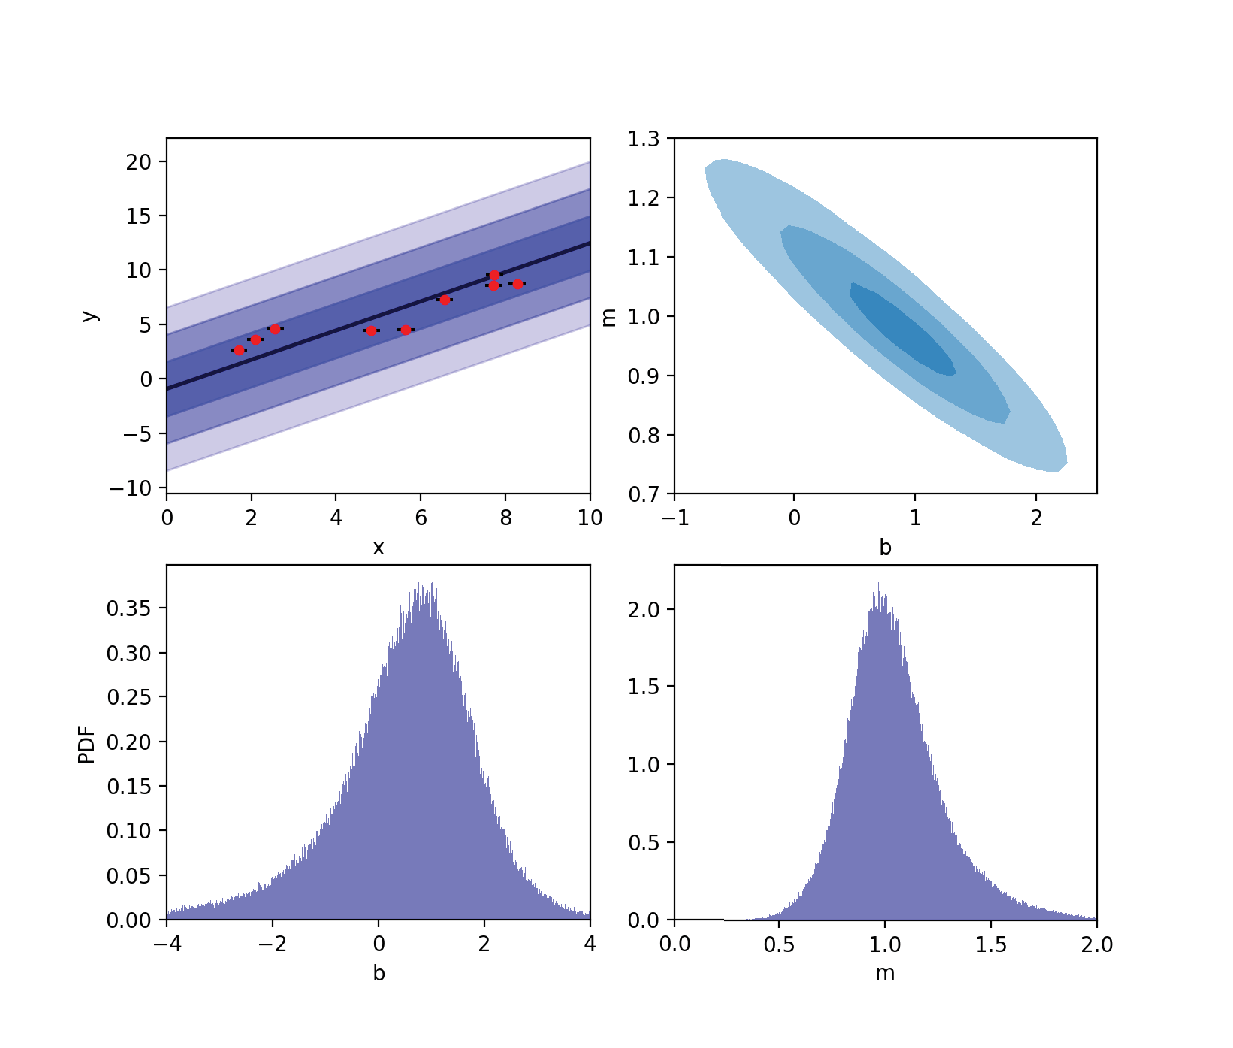
\includegraphics[width=1.0\linewidth]{figures/linfit_sloppy_3shadenoback.eps}
    \caption{Top left: Example extrinsic scatter-dominated dataset (red) with small $x-$ and $y-$ error bars (barely visible), alongside linear fit model distribution $y=mx+b$ with $1-$, $2-$ and $3\sigma$ slop confidence regions visible in blue. Top right: model parameter confidence ellipse with $1-$, $2-$ and $3\sigma$ regions shaded, generated from the posterior probability distributions for $b$ and $m$ found via MCMC, bottom.}
    \label{fig:linfit}
\end{figure}

I have now covered all of the essential parts of the TRK fitting suite, and provided an example of its usage. Before I  discuss the applications and more complicated examples of TRK fitting, and compare the method to similar algorithms, I will first examine further algorithms and options of the TRK suite, including an automated algorithm for the minimization of model parameter correlation for certain models, and allowing for asymmetric error bars and/or slop parameters.